\documentclass[10pt]{article}
\usepackage{icmlko}

\icmlmeta{IP 파운데이션 월드모델}{2}{언론은 일치하고, 우리가 나눈다}{수집 라벨의 스코프 판정과 타깃 분모 오류}

\begin{document}

\twocolumn[
\icmlheader

\begin{abstract}
연구 노트 1에서 우리는 주최자 발표 수치가 현장 게이트 계수보다 2.75배 높다는 것을 보였다.
그렇다면 발표 수치 자체는 얼마나 믿을 수 있는가? 언론 보도가 서로 얼마나 어긋나는가?
이 노트는 같은 행사를 두 매체 이상이 보도한 29쌍을 대조한다. 결과는 예상과 반대였다 ---
\textbf{언론 수치는 서로 잘 맞는다}. 두 보도의 차이는 중앙 1.15배이고, 89.7\%가 앞서 측정한
집계 기준 격차(2.75배)보다 작다. 크게 갈리는 소수(최대 12배)를 원문 인용문으로 추적하자,
그것은 측정 잡음이 아니라 \textbf{스코프와 시점의 차이}였다 --- 중간 집계 대 최종 집계,
단일 행사 대 다회차 합산, 부스 대 상권 전체. 이를 판정하는 분류기를 만들어 수집 라벨
328건에 적용한 결과 27건(8.2\%)이 타깃으로 쓸 수 없는 스코프였다. 더 중요한 것은
\textbf{타깃 분모의 오류}다. ``개장 3일 만에 10만 명''이라는 중간 집계 라벨을 전체 운영
기간 25일로 나누면 일평균이 4{,}000명으로 나오지만 실제로는 33{,}333명이다. 이런 분모
오류가 21건 있었고 \emph{전부 같은 방향}(과소평가)이었으며, 중앙 3.25배 어긋나 있었다.
언론 보도의 신뢰도를 문제 삼기 전에, 우리가 그 숫자를 어떤 창으로 나누는지를 먼저 확인해야 한다.
\end{abstract}
]

\section{앞선 노트에서 이어지는 물음}

연구 노트 1은 라벨 풀이 두 개의 서로 다른 물리량을 담고 있음을 보였다. 우리가 직접 운영한
팝업의 게이트 계수(중앙 519명/일)와 언론에 보도된 주최자 발표(중앙 1{,}429명/일)가
2.75배 벌어져 있었고, 같은 행사를 두 방식으로 잰 사례에서는 6.9배까지 갈렸다.

여기서 자연스러운 다음 물음이 나온다. \textbf{주최자 발표 수치 자체는 얼마나 안정적인가?}
만약 언론 보도가 서로 크게 어긋난다면, 2.75배라는 격차는 발표 수치의 잡음에 묻힐 것이다.
반대로 보도끼리 잘 맞는다면, 그 격차는 실재하는 체계적 편향이다.

이 물음에 답할 자료가 저장소에 있었다. 수집 과정에서 같은 행사를 다룬 다른 기사를 만나면
\texttt{alt\_figures} 필드에 원문 인용과 함께 기록해 두었다. 지금까지 이 필드는 참고
메모로만 쓰였고 분석된 적이 없다.

\section{같은 행사, 다른 매체}

\texttt{alt\_figures}를 가진 수집 라벨에서 (주 수치, 대안 수치) 쌍 31개를 추출했다.
그중 2쌍은 대안 수치에 ``단독 수치 아님'' 같은 스코프 경고가 이미 붙어 있어 제외하고,
남은 29쌍의 로그 비율 차이를 보았다.

\begin{figure}[t]\centering
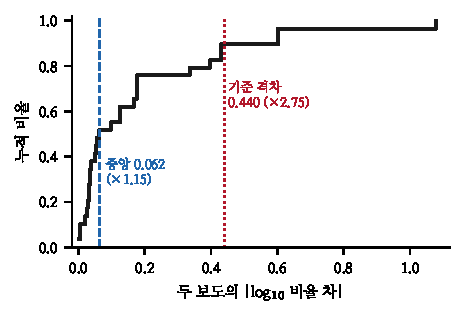
\includegraphics[width=\linewidth]{figs/press_agreement.pdf}
\caption{같은 행사를 보도한 두 수치의 차이(누적분포). 파란 파선은 중앙값,
붉은 점선은 연구 노트 1에서 측정한 집계 기준 격차. 보도의 89.7\%가 기준 격차보다
작게 어긋난다.}
\label{fig:agree}
\end{figure}

\claimx{언론 보도 수치는 서로 잘 맞는다. 두 보도의 차이는 중앙 $0.062\,\text{log}_{10}$
= 1.15배이고, 29쌍 중 26쌍(89.7\%)이 집계 기준 격차 2.75배보다 작게 어긋난다.}
{이 일치는 독립성이 아니라 \emph{복제}일 수 있다. 여러 매체가 같은 보도자료를 받아쓰면
수치가 같아진다. 각 인용문의 발행 매체와 날짜를 대조해 실제로 독립 취재인지 확인해야 한다.
표본도 29쌍뿐이다.}

이 결과는 연구 노트 1의 주장을 강화한다. 발표 수치의 자체 산포(1.15배)가 게이트 대비
격차(2.75배)보다 훨씬 작으므로, 그 격차는 잡음이 아니라 체계적 편향이다.

\section{크게 갈리는 소수는 왜 갈리는가}

그림~\ref{fig:agree}의 오른쪽 꼬리 --- 2.5배에서 12배까지 벌어진 5쌍 --- 을
원문 인용문으로 추적했다. 결과는 표~\ref{tab:tail}과 같다.

\begin{table}[t]\centering\tsize
\caption{크게 갈린 5쌍의 원인. 어느 것도 측정 오차가 아니다.}
\label{tab:tail}
\begin{tabular}{p{1.3cm}p{4.3cm}}
\toprule
차이 & 원인 \\
\midrule
12.0배 & 8일 누적 총계 대 일평균 --- \textbf{단위 차이} \\
4.0배 & 종료 직전 누적 대 개장 3일 누적 --- \textbf{시점 차이} \\
2.7배 & 더현대 단독 대 3개 점포 합계 --- \textbf{범위 차이} \\
2.5배 & 2023--2025 시리즈 누적 대 단년 10일 --- \textbf{기간 차이} \\
2.2배 & 전체 운영 기간 대 공식 행사 4일 --- \textbf{창 차이} \\
\bottomrule
\end{tabular}
\end{table}

\claimx{보도 간 큰 불일치는 측정 잡음이 아니라 스코프·시점의 차이다.
다섯 사례 전부 ``무엇을, 언제까지, 어디까지 세었는가''가 달랐다.}
{다섯 사례는 우리가 \texttt{alt\_figures}를 기록해 둔 것만 본 것이다. 기록하지 않은
불일치가 다른 성격일 수 있다. 다만 기록 여부가 원인 유형과 상관될 이유는 없어 보인다.}

\section{스코프 분류기}

위 유형을 원문 인용문에서 판정하는 규칙 기반 분류기를 만들었다. 판정 축은 넷이다.
\emph{중간 집계}(``개장 3일 만에''), \emph{전망치}(``넘어설 것으로''),
\emph{다회차 합산}(``세 차례 팝업''), \emph{범위 초과}(``잠실 일대'').
이 중 하나라도 걸리면 최종 집계 타깃으로 쓸 수 없다.

설계에서 한 가지를 특히 조심했다. \textbf{``누적''이라는 단어만으로는 판정할 수 없다.}
``8일간 누적 1만 2천 명''은 단일 행사의 정당한 총계이고, ``3회차 누적 17만 명''은 다른
행사들의 합이다. 회차나 점포를 세는 표현이 함께 있을 때만 다회차로 본다. 이 구분을 넣기
전 조잡한 규칙은 328건 중 118건(36\%)을 오염으로 잡았으나, 대부분 정당한 총계였다.

\begin{figure}[t]\centering
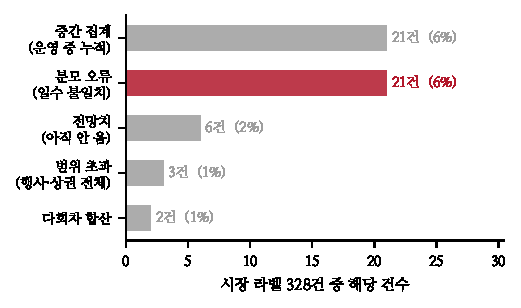
\includegraphics[width=\linewidth]{figs/scope_classes.pdf}
\caption{수집 라벨 328건의 스코프 판정. 붉은색은 타깃 분모가 잘못된 건으로,
스코프 오염과 별개의 결함이다.}
\label{fig:scope}
\end{figure}

\section{더 큰 문제 --- 타깃 분모}

스코프 분류 과정에서 예상하지 못한 결함이 드러났다. 인용문이 말하는 기간과 우리가 저장한
운영일수가 어긋나는 경우다.

우리 타깃은 총 방문객이 아니라 \emph{일평균} 방문객이다. 팝업의 운영 기간이 하루에서 두
달까지 다르므로 총계를 그대로 쓰면 기간 길이가 타깃을 지배한다. 그래서 총계를 운영일수로
나눈다. 그런데 라벨이 중간 집계인데 분모로 전체 기간을 쓰면 어떻게 되는가?

\begin{quote}\footnotesize
``지난 4월 잠실 월드몰 일대에서 진행된 포켓몬타운 2025 팝업은 \textbf{오픈 3일 만에}
방문객 10만 명을 돌파했다.''
\end{quote}

이 라벨의 저장된 운영일수는 25일이다. $100{,}000 \div 25 = 4{,}000$명/일로 계산되지만,
인용문이 말하는 것은 $100{,}000 \div 3 = 33{,}333$명/일이다. \textbf{8.3배 과소평가}다.

\begin{figure}[t]\centering
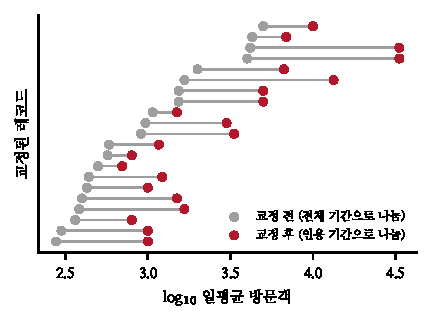
\includegraphics[width=\linewidth]{figs/denominator_fix.pdf}
\caption{분모 교정 전후. 각 선분이 레코드 하나이며, 회색이 교정 전, 붉은색이 교정 후다.
21건 전부 오른쪽으로 --- 즉 위로 --- 움직인다.}
\label{fig:denom}
\end{figure}

인용문에 기간이 명시된 105건 중 \textbf{21건}에서 저장 일수와 25\% 넘게 어긋났다.
그리고 \emph{전부 같은 방향}이었다 --- 저장 일수가 인용 일수보다 컸다.
교정 시 일평균이 중앙 $0.512\,\text{log}_{10}$(3.25배), 최대 $0.921$(8.3배) 올라간다.

\claimx{타깃 분모가 21건에서 틀렸고 전부 같은 방향이다. 중간 집계 라벨에 전체 운영
기간을 분모로 써서 일평균이 중앙 3.25배 과소평가됐다.}
{인용문의 기간 표현을 정규식으로 뽑았으므로 오독이 있을 수 있다. 특히 ``지난 3일까지
5일간''처럼 두 기간이 한 문장에 있으면 앞의 것을 잡는다. 21건은 수동 확인이 필요하다.}

\section{왜 이 방향인가}

21건이 모두 같은 방향이라는 사실이 우연이 아니다. 구조적 이유가 있다.

언론은 팝업이 \emph{화제일 때} 기사를 쓴다. 그 시점은 대개 운영 초반이고, 그래서 기사에
실리는 수치는 중간 집계다. 반면 우리 수집 파이프라인은 그 팝업의 \emph{전체} 운영 기간을
별도로 확인해 저장한다. 두 정보가 각각 옳지만 짝이 맞지 않는다.

이 구조는 편향의 방향을 고정한다. 중간 집계는 항상 전체 기간보다 짧은 창의 값이므로,
전체 기간으로 나누면 항상 과소평가된다. 무작위 오차가 아니라 \textbf{체계적 하향 편향}이다.

\section{결과의 크기}

솔직히 적으면, 이 교정이 풀 전체를 크게 바꾸지는 않는다. 328건 중 21건이므로
수집 라벨의 일평균 분포 중앙값은 움직이지 않았고, 표준편차가 0.538에서 0.549로
약간 넓어졌을 뿐이다.

그러나 개별 레코드 수준에서는 최대 8.3배의 교정이다. 그리고 이 21건은 우연히 모인 것이
아니라 ``화제성이 높아 초기에 기사화된 팝업''이라는 특정 유형이다. 즉 \textbf{교정 전
데이터는 흥행한 팝업의 일평균을 체계적으로 낮게 기록하고 있었다}. 수요를 예측하려는
모델에게 이는 무해한 잡음이 아니다.

\section{한계와 다음 단계}

\paragraph{확정}
언론 보도 수치는 서로 잘 맞는다(중앙 1.15배). 따라서 연구 노트 1의 2.75배 격차는
발표 수치의 잡음이 아니라 체계적 편향이다. 큰 불일치는 스코프·시점 차이이며 판정 가능하다.
타깃 분모가 21건에서 틀렸고 전부 같은 방향이다.

\paragraph{열린 것}
보도 간 일치가 독립 취재의 결과인지 보도자료 복제의 결과인지 구분하지 못했다.
분류기는 규칙 기반이므로 인용문이 짧거나 모호하면 판정하지 못한다 --- 328건 중 기간이
명시된 것은 105건뿐이다. 나머지 223건의 분모는 검증되지 않은 채로 남아 있다.

\paragraph{다음 단계}
(1) 인용문의 발행 매체와 날짜를 대조해 보도 독립성을 확인한다.
(2) 기간이 명시되지 않은 223건에 대해 원문 URL을 다시 열어 창을 확정한다.
(3) 스코프가 확정된 라벨만으로 학습 풀을 재구성하고, 그 위에서 모델을 다시 검정한다.
연구 노트 1과 2가 함께 말하는 것은, 이 재구성이 끝나기 전의 모든 모델 비교가
해석 불가능하다는 것이다.

\vspace{0.7em}
\hrule
\vspace{0.4em}
{\footnotesize\color{black!60}
분류기 구현은 \texttt{ingest/market\_scope.py}, 그림 생성은 \texttt{paper/figs.py}에 있으며
모두 저장소 데이터에서 직접 계산한다. 라벨이 갱신되면 수치도 함께 바뀐다.}

\end{document}
